\documentclass[a4paper,12pt]{article}

\usepackage{graphicx}
\usepackage{epsfig,subfigure}
\usepackage[%dvipdfm,
            CJKbookmarks=true,%
            bookmarksnumbered=true,
            bookmarksopen=true, %Collapse all bookmarks at pdf start view
            pdfauthor=kmc,
            pdfcreator={LaTex with hyperref package},
            pdftitle=trudge,
            colorlinks,%
            linkcolor=blue,%
            hyperindex,%
            plainpages=false,%
            pdfstartview=FitH,
            linktocpage=true,
            citecolor=blue,
            hyperindex=true
            ]{hyperref}
\usepackage{listings}
\lstset{language=C}

\addtolength{\textwidth}{50pt}
\addtolength{\evensidemargin}{-25pt}
\addtolength{\oddsidemargin}{-25pt}

\def\displayandname#1{\rlap{$\displaystyle\csname #1\endcsname$}%
                      \qquad \texttt{\char92 #1}}
\def\mathlexicon#1{$$\vcenter{\halign{\displayandname{##}\hfil&&\qquad
                   \displayandname{##}\hfil\cr #1}}$$}

\newpage
\begin{document}

\title{ Notes for the Development of CertiKOS Prototype }
%\author{Liang Gu}
%\date{2nd Edition\\[3pt]
%Copyright \copyright\ David R. Wilkins 1995}
\maketitle

\tableofcontents

\newpage
\section{About CertiKOS }

CertiKOS (Certified Kit Operating System) may refer to our project: applying new advances
in certified software \cite{certifiedsoftware} to the development of a novel OS kernel. For more information about the whole project, please check  the project tech report \cite{CertiKOSReport}. In this document, we mostly use CertiKOS to refer to the prototype of the OS kernel.

For the long term,  our CertiKOS is supposed to offer features as follows: safe and application-specific extensibility, provable security properties with information flow control, and accountability and recovery from hardware or application failures. The implementation will have different stages to provide these features. At current stage, CertiKOS is trying to provide some demonstration features (Section \ref{sec:currentstage}). This document will be updated later with the progress of implementation.


\section{CertiKOS at Current Stage}
\label{sec:currentstage}


\subsection{Overview}
\begin{figure}[!ht]
 \centerline{
 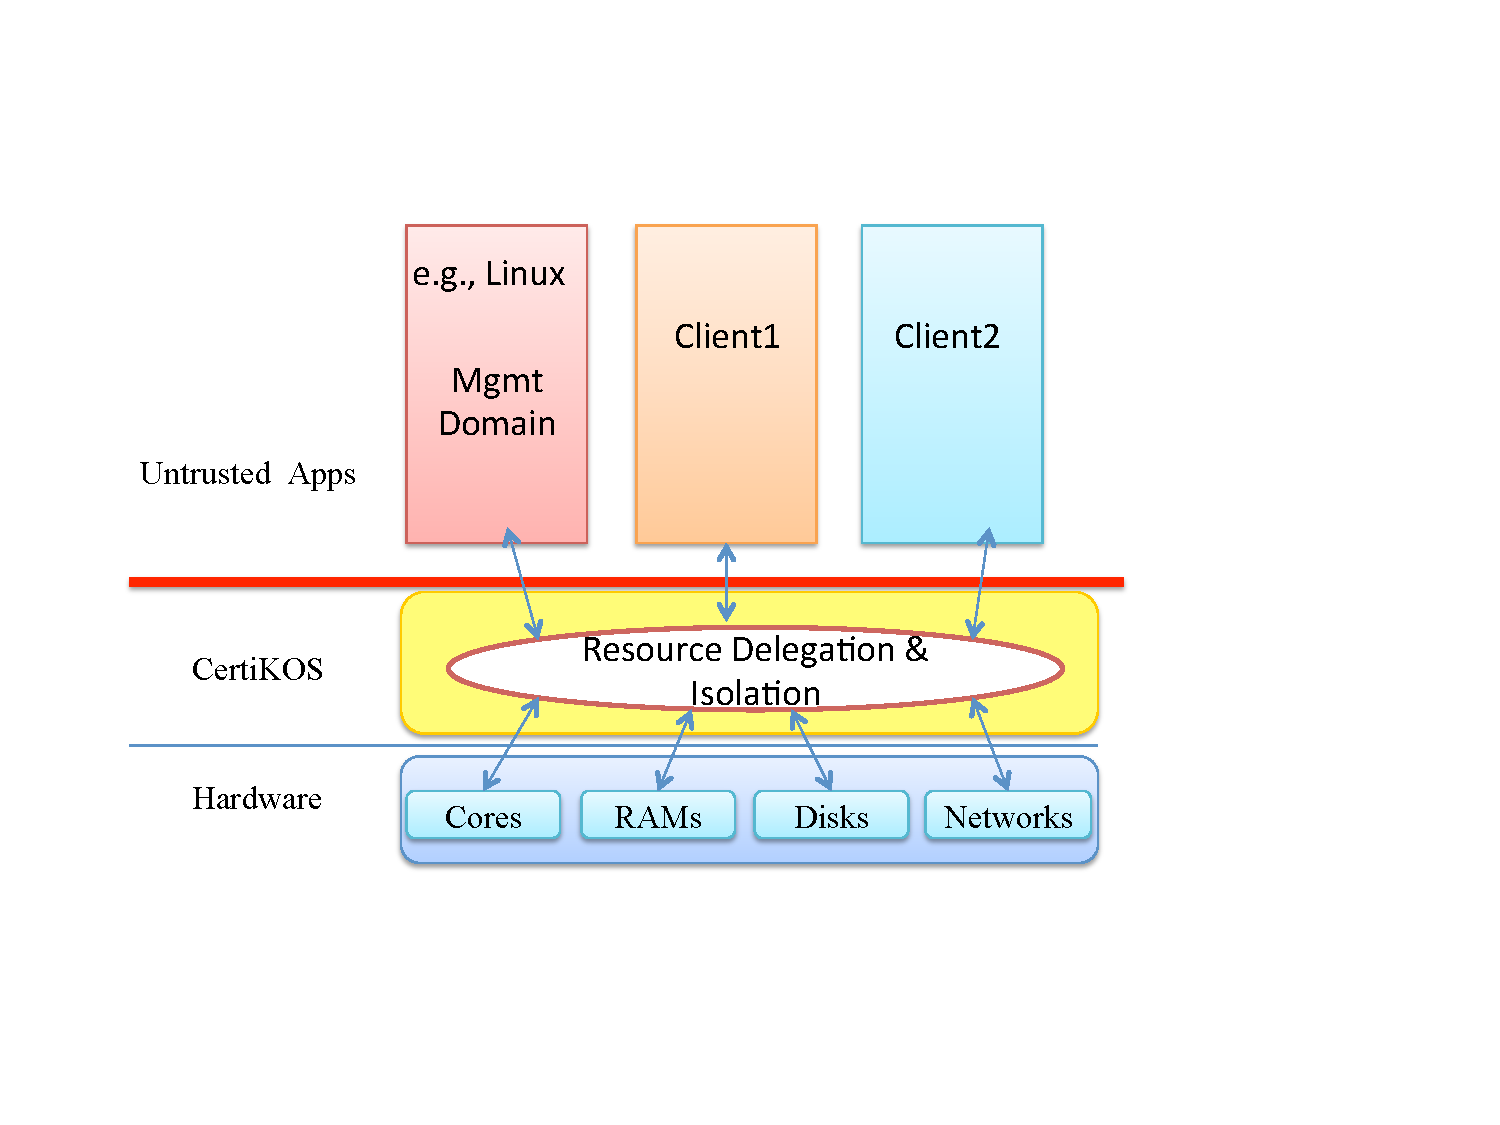
\includegraphics[width=0.6\textwidth]{overview.pdf}}
 \caption{Overview of CertiKOS at current stage} \label{fig:overview}
\end{figure}

The overview of current CertiKOS  is shown in Figure \ref{fig:overview}.  It is trying to provide demonstration features as follows:
\begin{itemize}
\item  Abstract resources for cloud computing, including CPU cores, RAMs, Disk, and Networks
\item  Separate the resource management from usage, move resource management facilities up to the untrusted application layer
\item  Support legacy OS as the management software
\item  Provide isolated execution environment to protect the execution of mission-critical (or security sensitive) operations,  according to the request from the application layer processes.
\end{itemize}

\subsection{Typical Usages }
We use several usage cases to specifically explain these above features.

\subsubsection{Resource Management}
Manage software runs at the untrusted application layer and it provides interfaces for administrator to manage the allocation of resources to each application.  As shown in Figure \ref{fig:resourcemgmt}, manage software instructs  CertiKOS to allocate  or revoke resources for applications.   Each application will be authorized to access its own resources, including memory space, cpu cores, disk and network.
\begin{figure}[!ht]
 \centerline{
 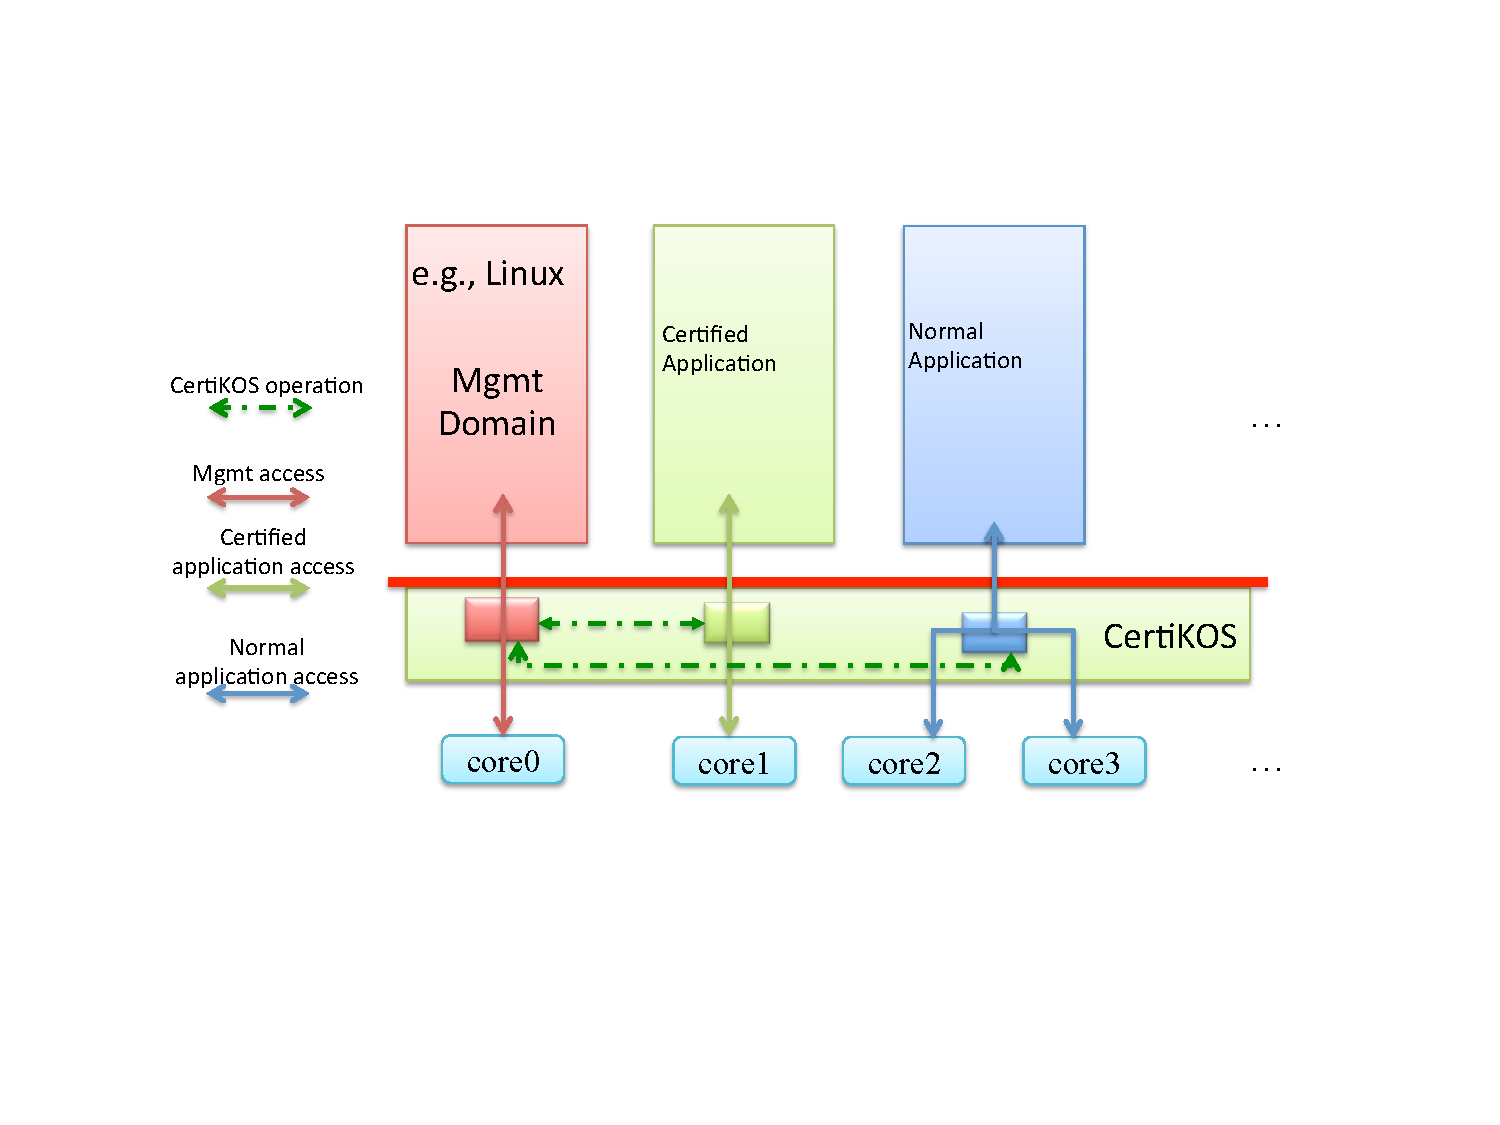
\includegraphics[width=0.7\textwidth]{certikos_resource_mgmt}}
 \caption{Resource Management} \label{fig:resourcemgmt}
\end{figure}


\subsubsection{Isolation}

Protect applications from each other, including management software.  The management software and other applications are equally treated as untrusted applications. As shown in Figure \ref{fig:isolation}, CertiKOS separately allocates memory spaces for them  and they can only access their own space.  The management software can manage the ownership of these resources, but it can not access these resources.   Applications are protected from each other and accessing among each other are prohibited.
\begin{figure}[!ht]
 \centerline{
 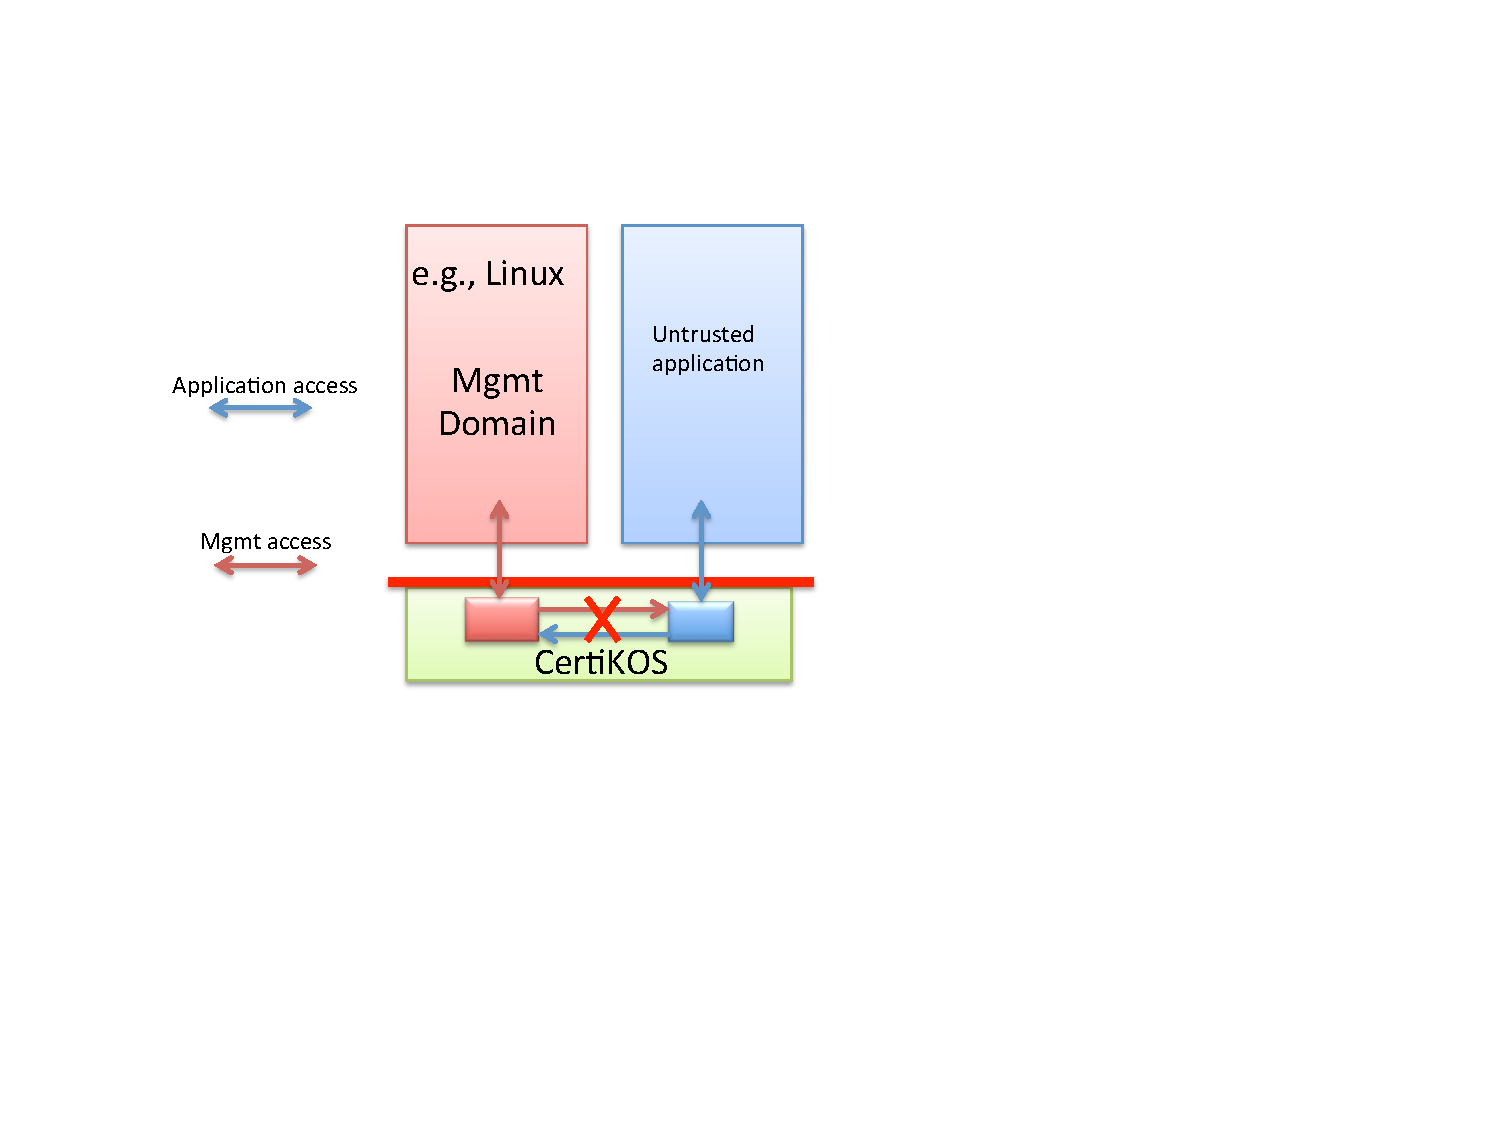
\includegraphics[width=0.4\textwidth]{certikos_isolation}}
 \caption{Isolation among untrusted applications} \label{fig:isolation}
\end{figure}

\subsubsection{Execute Certified Applications}
As shown in Figure \ref{fig:certified_ap}, certified applications can run on top of CertiKOS as normal applications and it will be protected from the management software and other applications.

\begin{figure}[!ht]
 \centerline{
 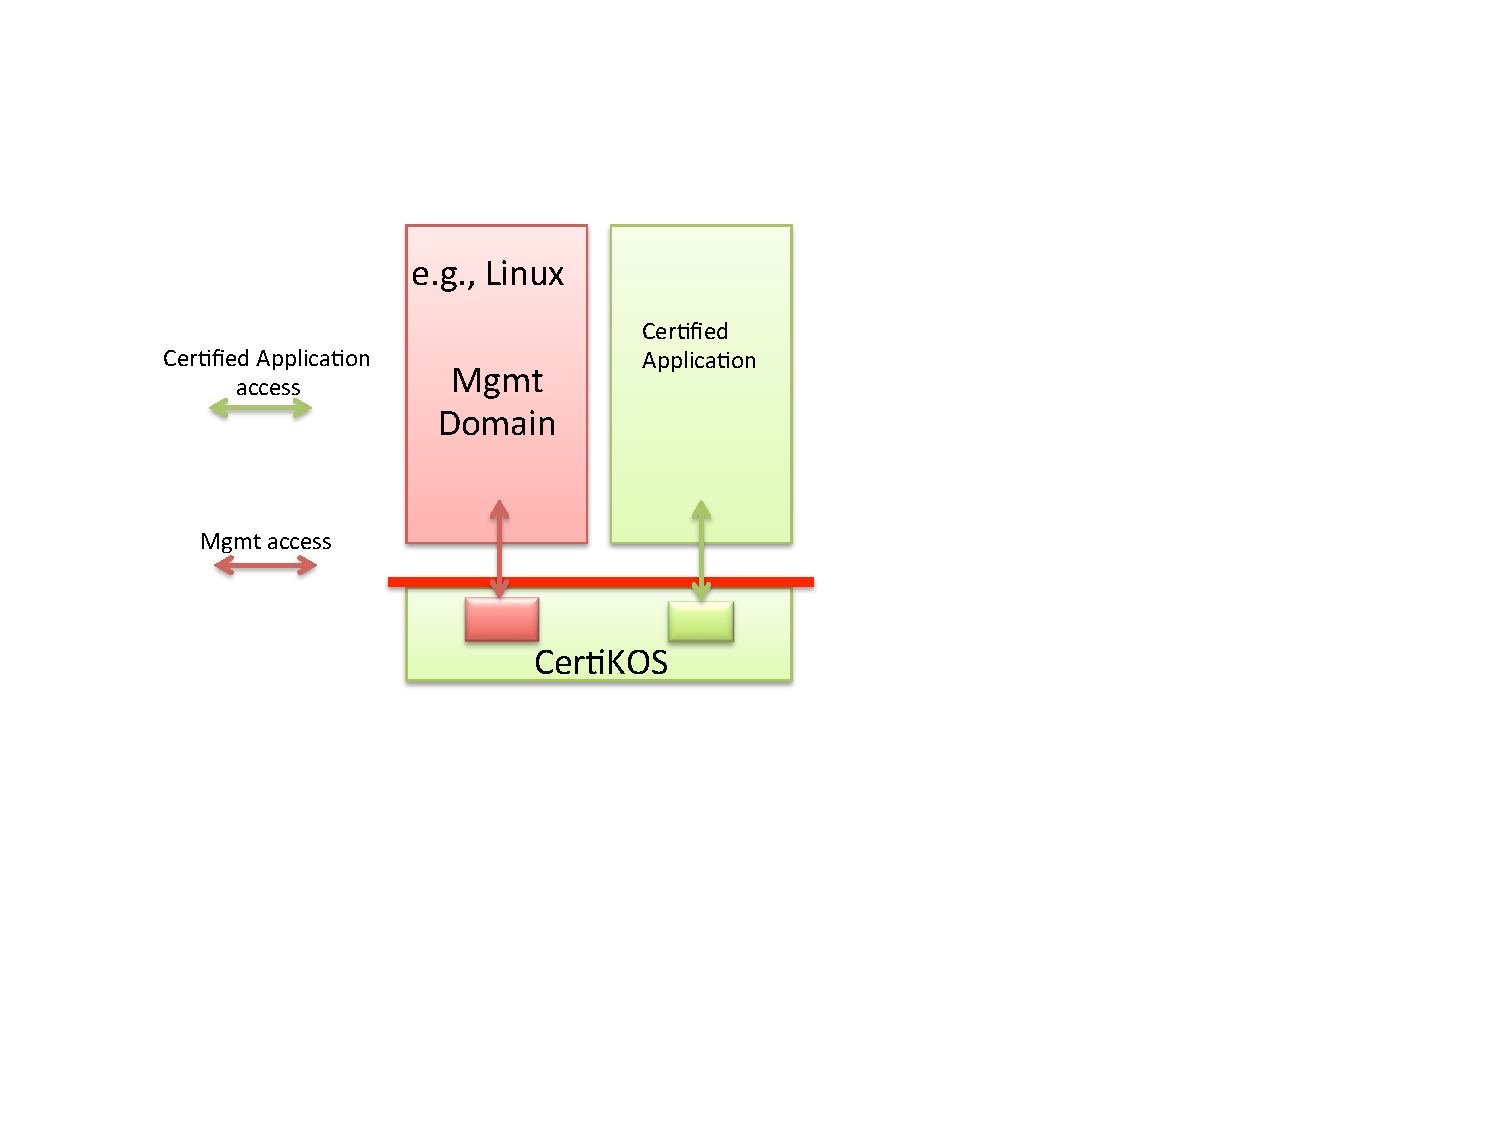
\includegraphics[width=0.4\textwidth]{certikos_certified_ap}}
 \caption{Certified Application on CertiKOS} \label{fig:certified_ap}
\end{figure}

\subsubsection{Protect Security Operations in Applications}
Many applications involve security related operations, in which sensitive information might be revealed, such as private key, credit card number,  social security number, etc. These applications may run atop of untrusted OS, and these security information can not be protected from compromised OS.

With Hardware-based Virtualization support, CertiKOS can provides isolated execution environment for these security related operations.  As shown in Figure \ref{fig:sandbox}, The legacy OS and applications can run on top of CertiKOS.  When the application tries to execute security sensitive operations,  CertiKOS  will setup a separated space for the security code block to execute.  After finishing execution in the isolated space, CertiKOS will return the result to the application and it  will continue execution in the legacy OS.



\begin{figure}[!ht]
 \centerline{
 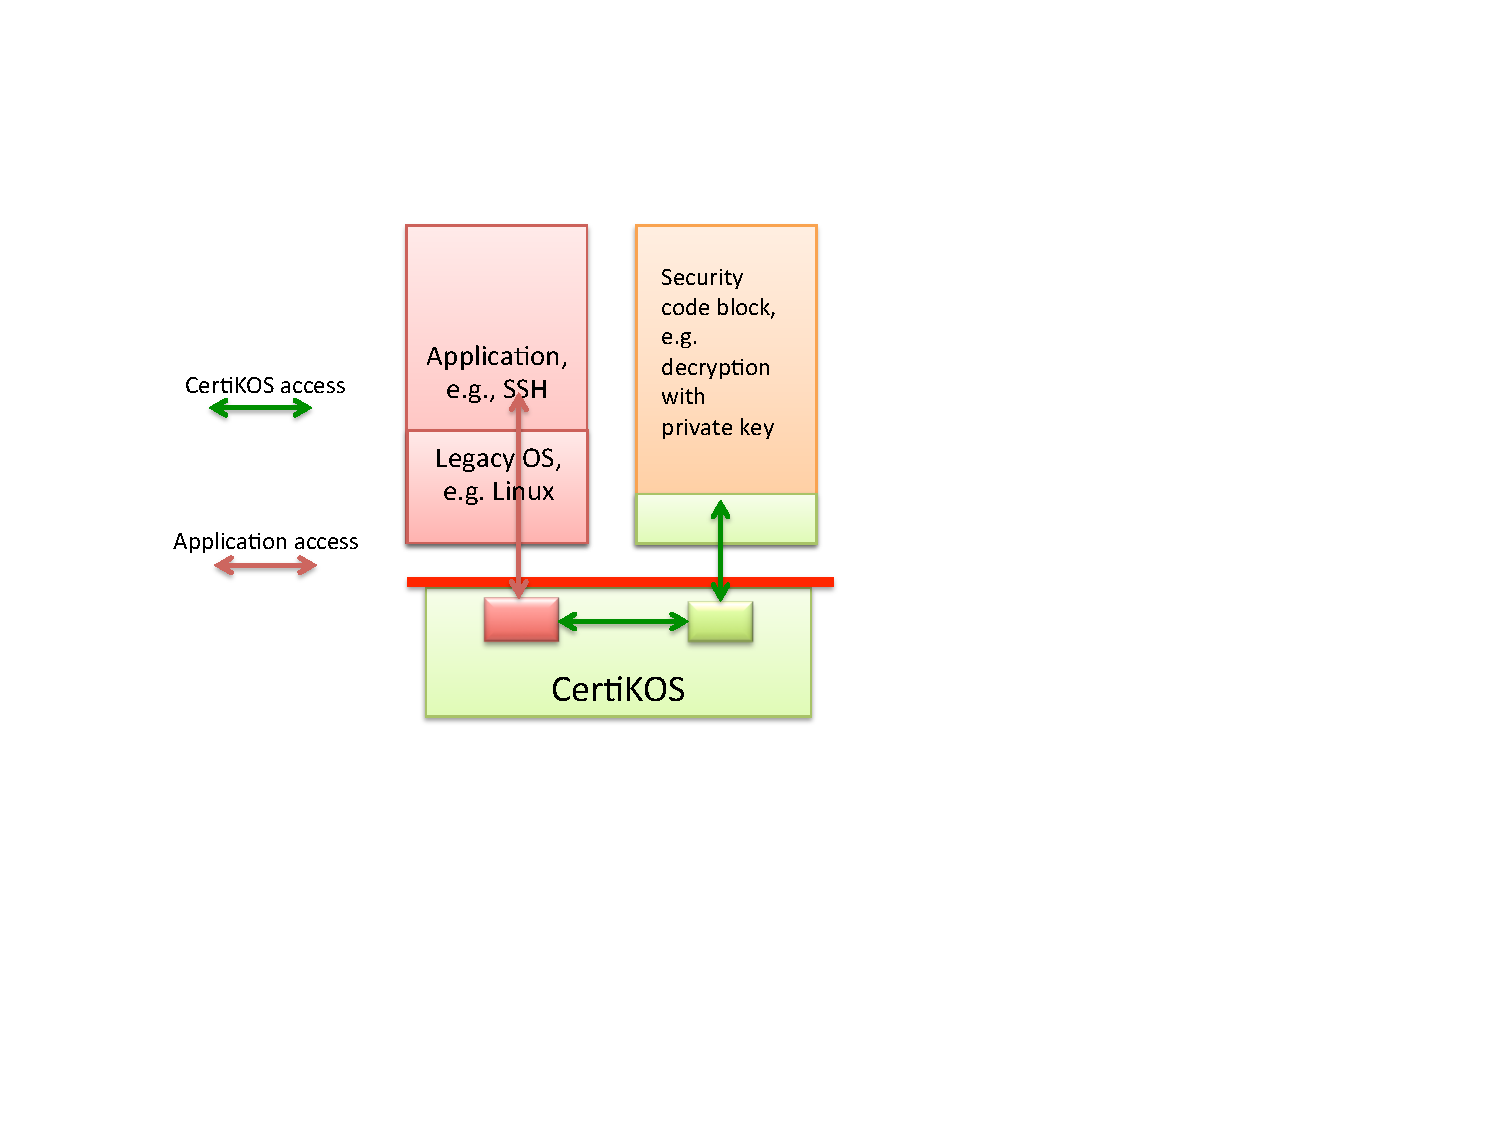
\includegraphics[width=0.4\textwidth]{certikos_sandbox}}
 \caption{Isolated Execution for Security Operations of Applications} \label{fig:sandbox}
\end{figure}

\section{CertiKOS Implementation}

\subsection{CertiKOS Framework}

\begin{figure}[!ht]
 \centerline{
 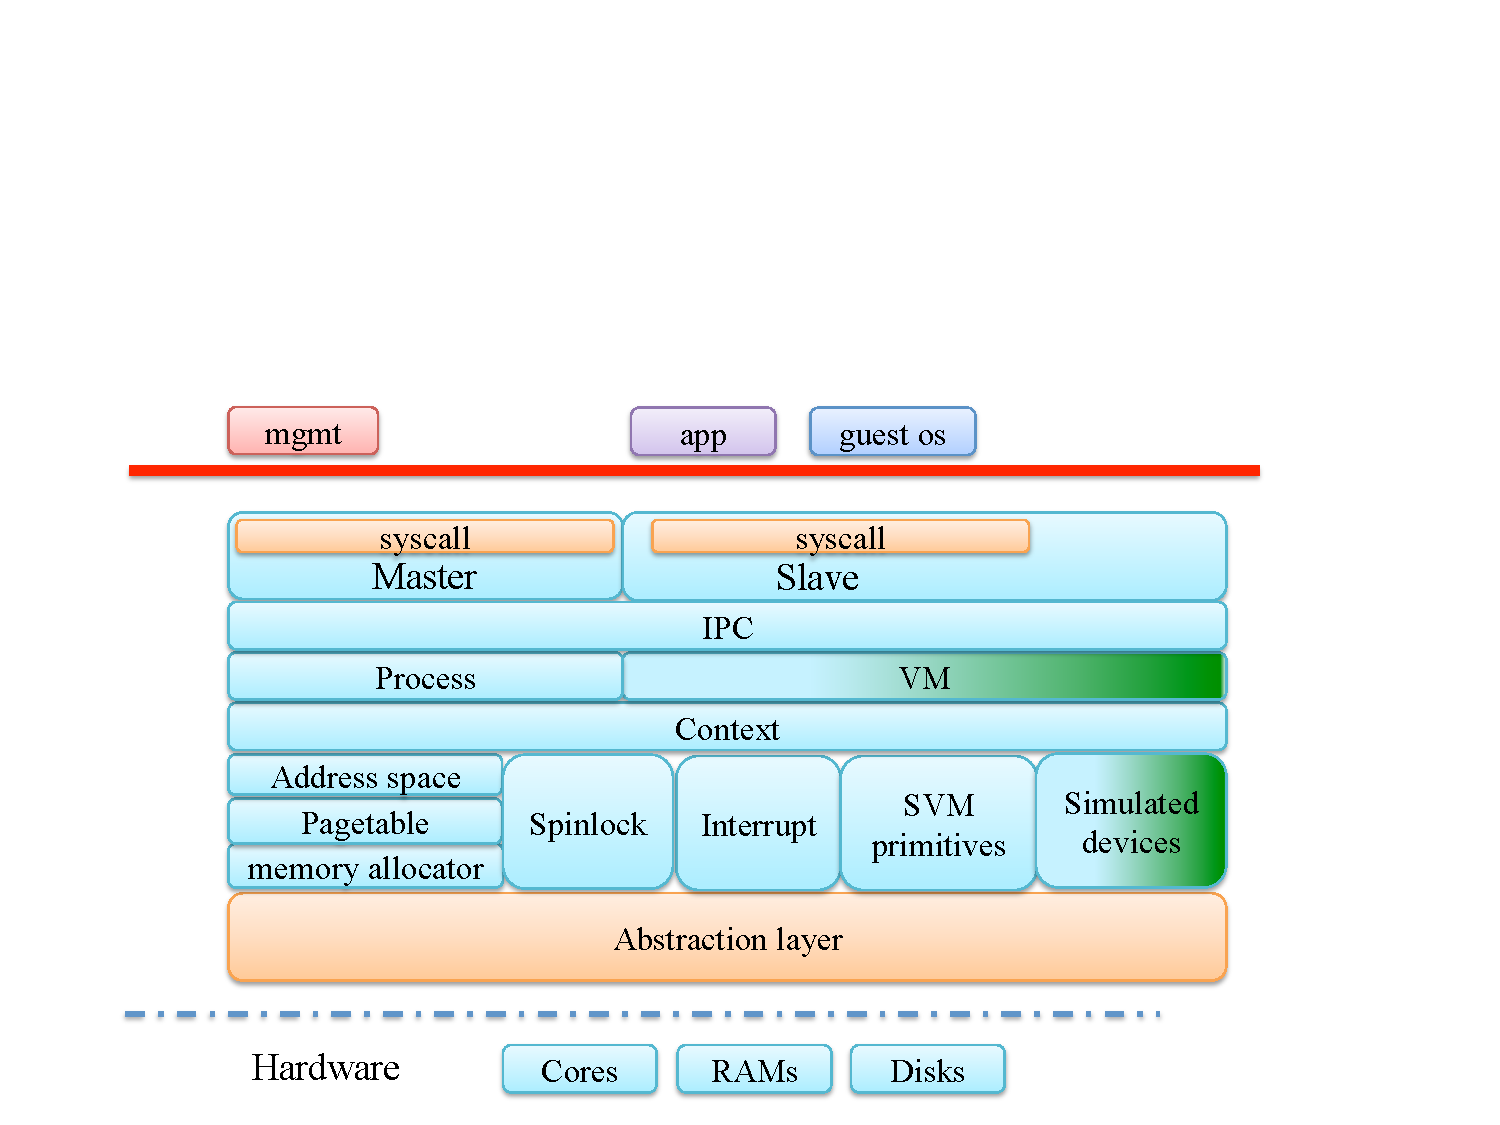
\includegraphics[width=0.8\textwidth]{certikos_framework}}
 \caption{CertiKOS Framework} \label{fig:framework}
\end{figure}

Current version of CertiKOS  is organized as in Figure \ref{fig:framework}. Upper layers depend on(invoke) lower layers components.  Ported from PIOS \cite{PIOS}, CertiKOS can now support the management of normal processes. To support legacy OS as the management software, CertiKOS will leverage the Hardware-based Virtualization. The current implementation work is mostly focusing on SVM based virtualization support for legacy OS.  These components with mixed color of Green and Blue denotes these undergoing implementation.

\subsection{Memory Management}

\subsubsection{address mode for host}

\subsubsection{memory space for guest os }

[TOFILL]
\subsection{CPU Core Management}

CPU core scheduling.
[TOFILL]


\subsection{ Hardware-based Virtualization}
AMD SVM provides the processor instruction support to enhance the implementation of Virtual Machine Monitor. These key features for virtualization support in CertiKOS include:  Nested Paging,  Interception.  For more specific info, please check specification \cite{AMD64, AMDSVM}.

\subsubsection{Virtual Machine Control}
VMCB  (Virtual Machine Control Block ) is the most important data structure in SVM.  It contains all information for the guest to run.  The VMM controls the  execution, resumption and interception of the guest os by setting the VMCB accordingly.  For more details, please refer to the SVM specification.

\begin{figure}[!ht]
 \centerline{
 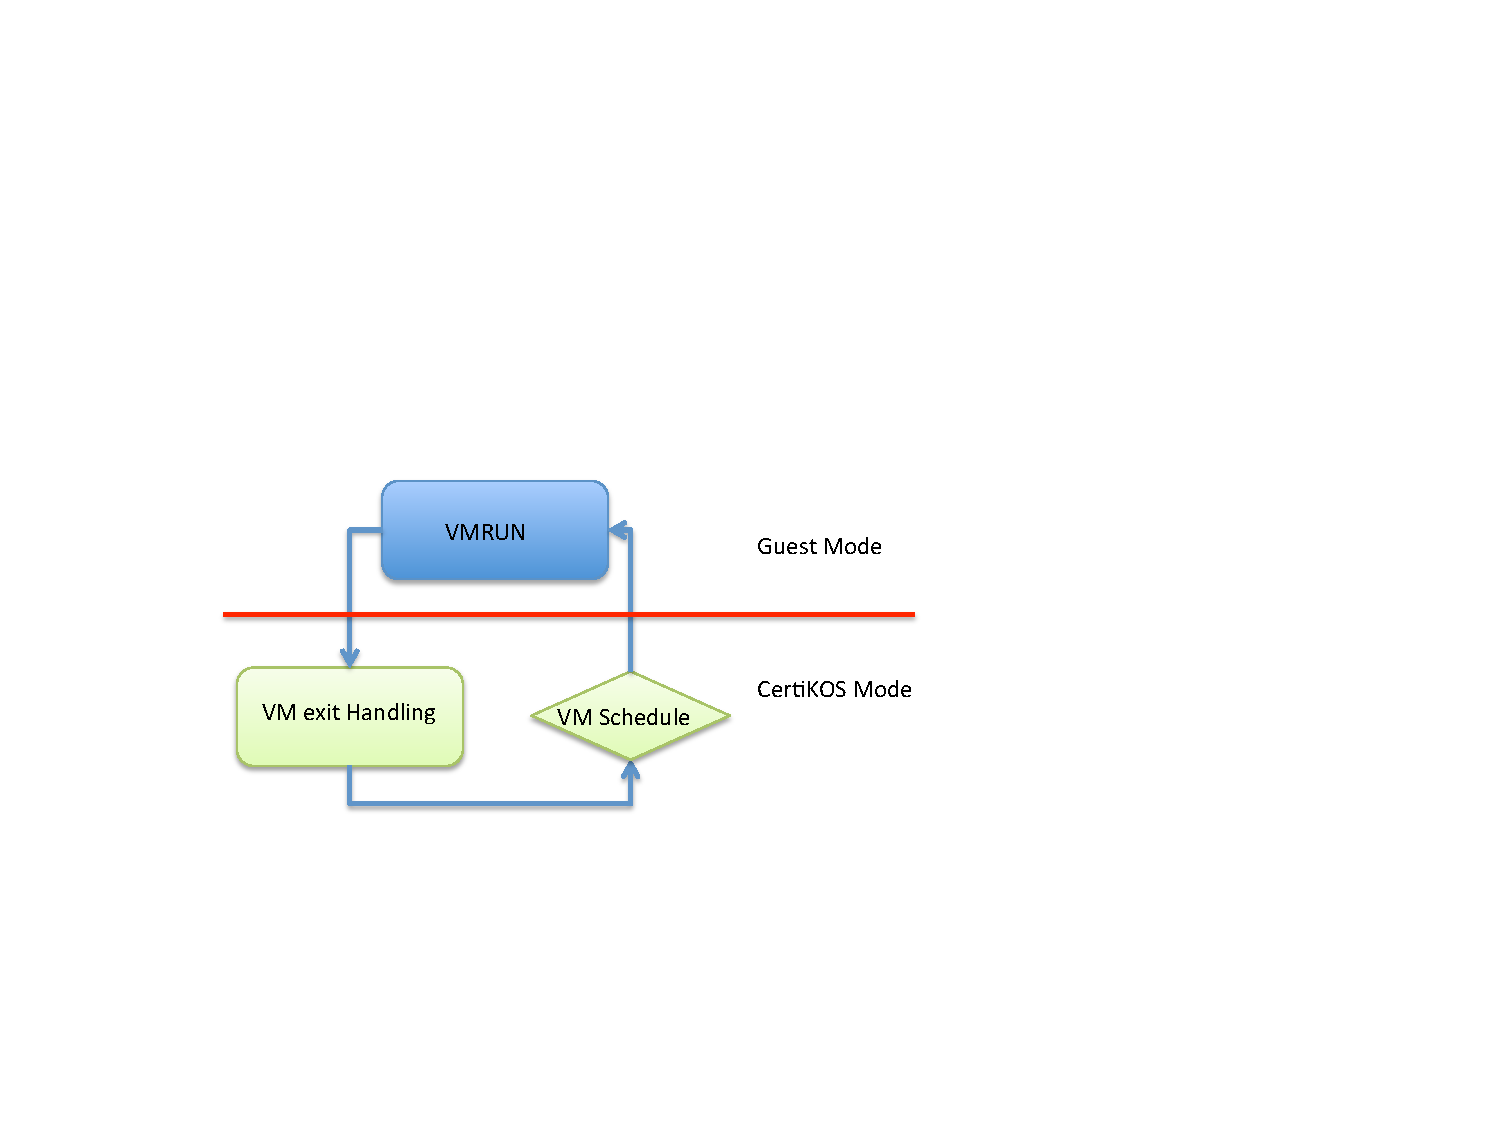
\includegraphics[width=0.6\textwidth]{vm_flow}}
 \caption{Execution Flow of VMs} \label{fig:vmflow}
\end{figure}


The basic execution flow of AMD SVM based VMM is shown as in Figure \ref{fig:vmflow}.When a VM is scheduled to run, its VMCB address will  be transferred to VMRUN instruction. Then the VMRUN will continue the execution of the VM, until exceptions or interception happen in the VM.   VM exit Handling will specifically deal with the exit events according to its exit code. After the exit handling, the VM will be ready for scheduling again.



\subsubsection{Nested Paging}
With Nested Paging in SVM, VMM does not  have to maintain a shadow page table for the guest OS.

\begin{figure}[!ht]
 \centerline{
 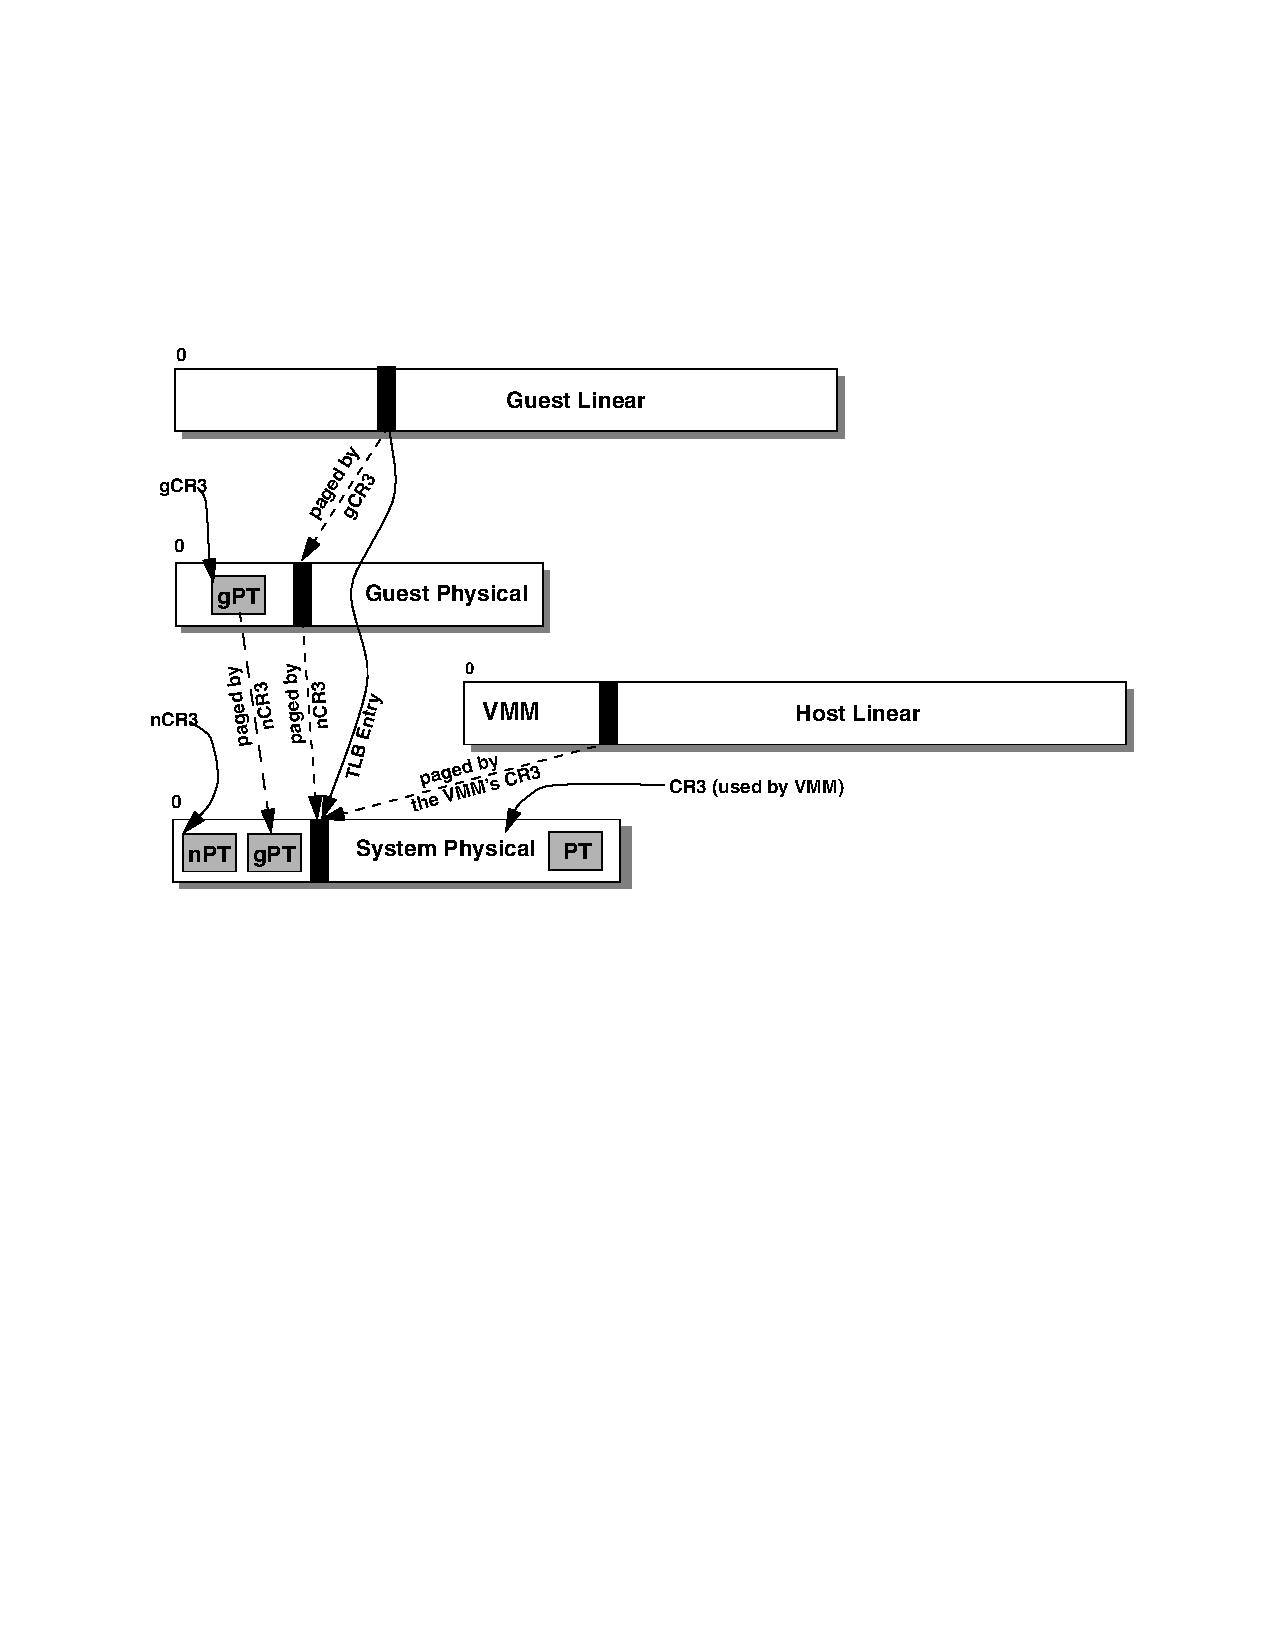
\includegraphics[width=0.8\textwidth]{NestedPaging}}
 \caption{Address Translating with Nested Paging} \label{fig:nestedpaging}
\end{figure}

With nested paging enabled, two levels of address translation are applied; Shown as in Figure \ref{fig:nestedpaging}.

\begin{itemize} \item Both guest and host levels have their own copy of CR3, referred to as gCR3 and nCR3,
respectively.
\item Guest page tables (gPT) map guest linear addresses to guest physical addresses. The guest page tables are in guest physical memory, and are pointed to by gCR3.
\item	Nested page tables (nPT) map guest physical addresses to system physical addresses. The nested page tables are in system physical memory, and are pointed to by nCR3.
\item The most-recently used translations from guest linear to system physical address are cached in the TLB and used on subsequent guest accesses.
\end{itemize}

\paragraph{Usage of Nested Paging}

First create a  layered page tables according to the addressing mode.  Then set the page table according to the memory space setting for the guest OS.  For example, mapping some physical memory region for the guest os, including some parts of the lower 1MB memory space.  Then configure the VMCB.

\subsubsection{Interception}
By setting the control data structure in VMCB, the running guest with VMRUN can be intercepted when its execution satisfies the interception condition.  CertiKOS uses interception to handle events of guest OS, including IO handling, Interrupt handling. Following interceptions are currently concerned in our implementation:
\begin{itemize}
\item IO
\item Interrupts
\item Debug
\item Page Fault
\item  Other exceptions

\end{itemize}


\subsection{Device Simulation for Supporting Legacy OS }
To support the co-exist of CertiKOS and up layer legacy OS, it requires virtualization for critical devices.  Previous implementation of CertiKOS simply exposes all hardwares to the legacy OS and it will change the settings of some critical devices, like PIC chips. This results the failure after switching back from legacy OS to CertiKOS.

We are now working at two directions:  Configure and test the legacy OS to identify the minimum  set of hardware devices, and enable the booting of ttyLinux with SVM on physical platform; Implement the simulation of these necessary devices one by one.

According to our current observation, following devices need to be specifically concerned: DMA, PIC, PCI, APIC, IOAPIC.

\subsubsection{Test CertiKOS on Physical Platform}
The previous versions of CertiKOS are mostly running on SimNow. We leverage the powerful debugging function of SimNow to quickly search and fix the errors and bugs in CertiKOS. However, the real physical platforms may have some subtle differences from SimNow, which cause CertiKOS cannot function properly in the real world. Thus, an indispensable part of our work is to port and test CertiKOS on the physical platform. The first two phases is to boot CertiKOS on the physical platform, and boot a guest OS on CertiKOS. In the future, we need to do more test and fixes to let the CertiKOS and the guest OS work properly other than just bootstrap.

\paragraph{Boot CertiKOS}
Current version CertiKOS must work on a SMP platform, because it requires the management OS and client applications run on different processor cores. Thus, CertiKOS checks whether it is running on a SMP platform when booting. If not, CertiKOS will not work properly, {\it e.g.} panic on UP platform. Previous versions of CertiKOS follow Intel Multiprocessor Specification\cite{MP} to detect and mange multiprocessors, {\it i.e} through {\it MPT}({\it MultiProcessor Table}). However, \cite{MP} is actually deprecated and lots of recent machines do not provide MPT any more. CertiKOS can not boot on these machines consequently. The resolution is turning to {\it ACPI}({\it Advanced Configuration and Power Interface}), which is the new standard. The legacy MPT code now works as a fallback method for the old platforms follow Intel Multiprocessor Specification other than ACPI. After fixing this error, CertiKOS can now boot on our physical machine. Still we need to test on more physical platforms.

\paragraph{Boot Guest OS (TTY Linux)}
The subtle differences between SimNow and the physical platform also cause the failure of booting TTY Linux as the guest OS in the real world. After bootloader loads the linux kernel, the kernel will first detect the hardware, set up the memory layout for the physical memory, and then create the data structures for paging, etc. Then is the non-architecture specific booting procedure, {\it i.e.} setting up interrupts, perform memory configuration and load the initial RAM disk. In the end of this procedure, the kernel will start an idle task (a user thread).

Currently TTY Linux can pass all architecture specific booting procedure, but it maybe stuck at some places in the non-architecture specific booting procedure, such as the point starting the idle task. Though the later procedure is named as {\it non-architecture specific}, some functions invoked in this procedure still depend on the hardware. Take the starting idle task as an example. The primary function of idle task is ``idle''. However, the implementation of ``idle'' depends on the features of the processors. In this case, the feature is called {\it C1E}. The hardware configuration we use in SimNow does not support C1E. While the real processors have this feature, so CertiKOS is stuck in the real world, though it works properly in the simulator.

We follow such steps to resolve these problems:
\begin{enumerate}
\item Disable the feature caused the problem. If it works, then go to the next problem; otherwise, take the second step.
\item Simulate the feature in SimNow, {\it i.e.} either implementing the feature in SimNow, or allowing the guest OS to access the feature of the hardware.
\end{enumerate}


\subsubsection{IO Port Interception for Devices Simulation}
Some devices are accessed via IO ports. Their simulations can be implemented with I/O interceptions.


\paragraph{List of critical devices}
By enabling the interception of all IO accessing,  we noticed that following IO ports are accessed by the guest domain when it boots ttyLinux with Grub:
\begin{itemize}
\item DMA: 0x80
\item PIC: 0xa0 0x20 0x21
\item 0xed

\item CGA: 0x3d4 0x3d5
\item PCI:  0xcf8 0xcfc
\item 0x1020
\end{itemize}

By Intercepting IO operations on these ports, we can implement the simulation of these devices while handling vm exit events.

\subsubsection{IO interception  handling for device simulation}


For simplicity, we currently introduce IO handling in the CertiKOS kernel, as  in Figure \ref{fig:iohandling}.  When a the guest OS is going to access a simulated device, CertiKOS intercepts the operation. It either sets the simulated data structure with these setting from guest OS, or returns the configuration from these simulated data structure to the guest OS.

\begin{figure}[!ht]
 \centerline{
 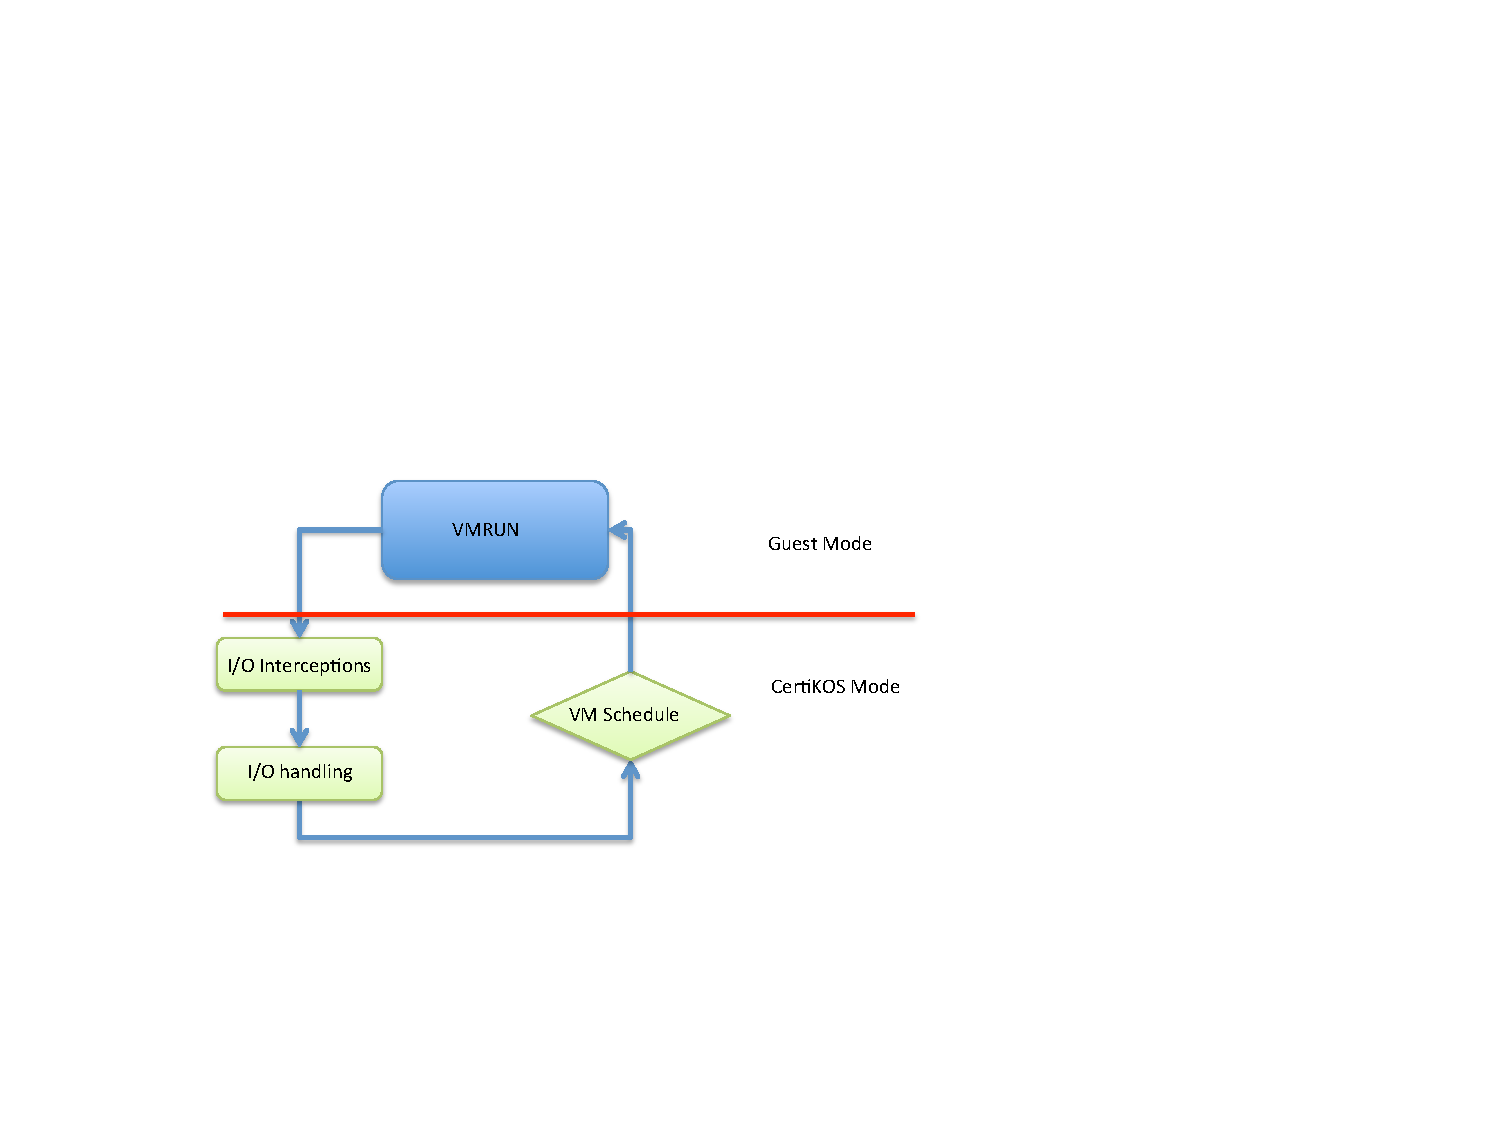
\includegraphics[width=0.7\textwidth]{IO_handling}}
 \caption{IO handling for VM at kernel mode} \label{fig:iohandling}
\end{figure}

For the long term, we will move IO handling up to application layer,  as in Figure \ref{fig:iohandling2}
\begin{figure}[!ht]
 \centerline{
 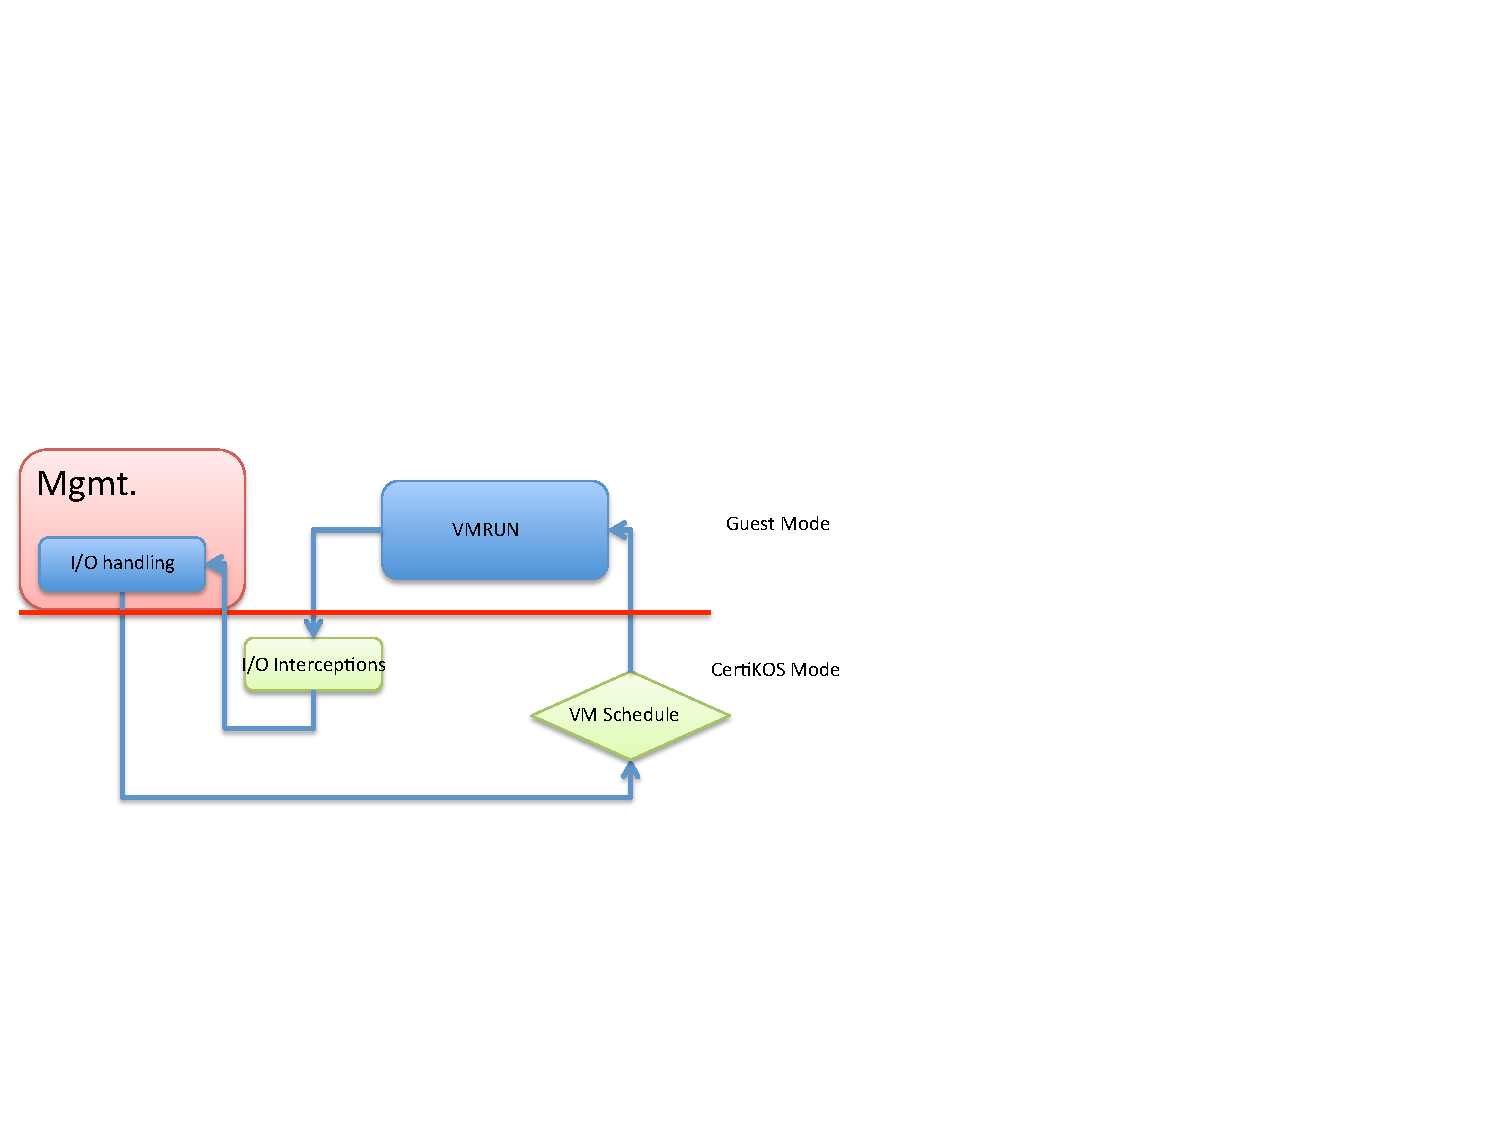
\includegraphics[width=0.7\textwidth]{IO_handling2}}
 \caption{IO handling for VM at guest mode} \label{fig:iohandling2}
\end{figure}



\subsubsection{PIC}
We first try to support guest domain with only PIC interrupt mode. The PIC interrupt mode is shown as in Figure \ref{fig:picmode}.  From the point view of guest OS, it can only see and access these virtualized 8259 pic chips. So we need to modify the multiprocessor  configuration  presented to the guest OS.   In recent years, these latest hardware platforms have already employed the ACPI specification for providing MP configuration \cite{ACPI4}.
\begin{figure}[!ht]
 \centerline{
 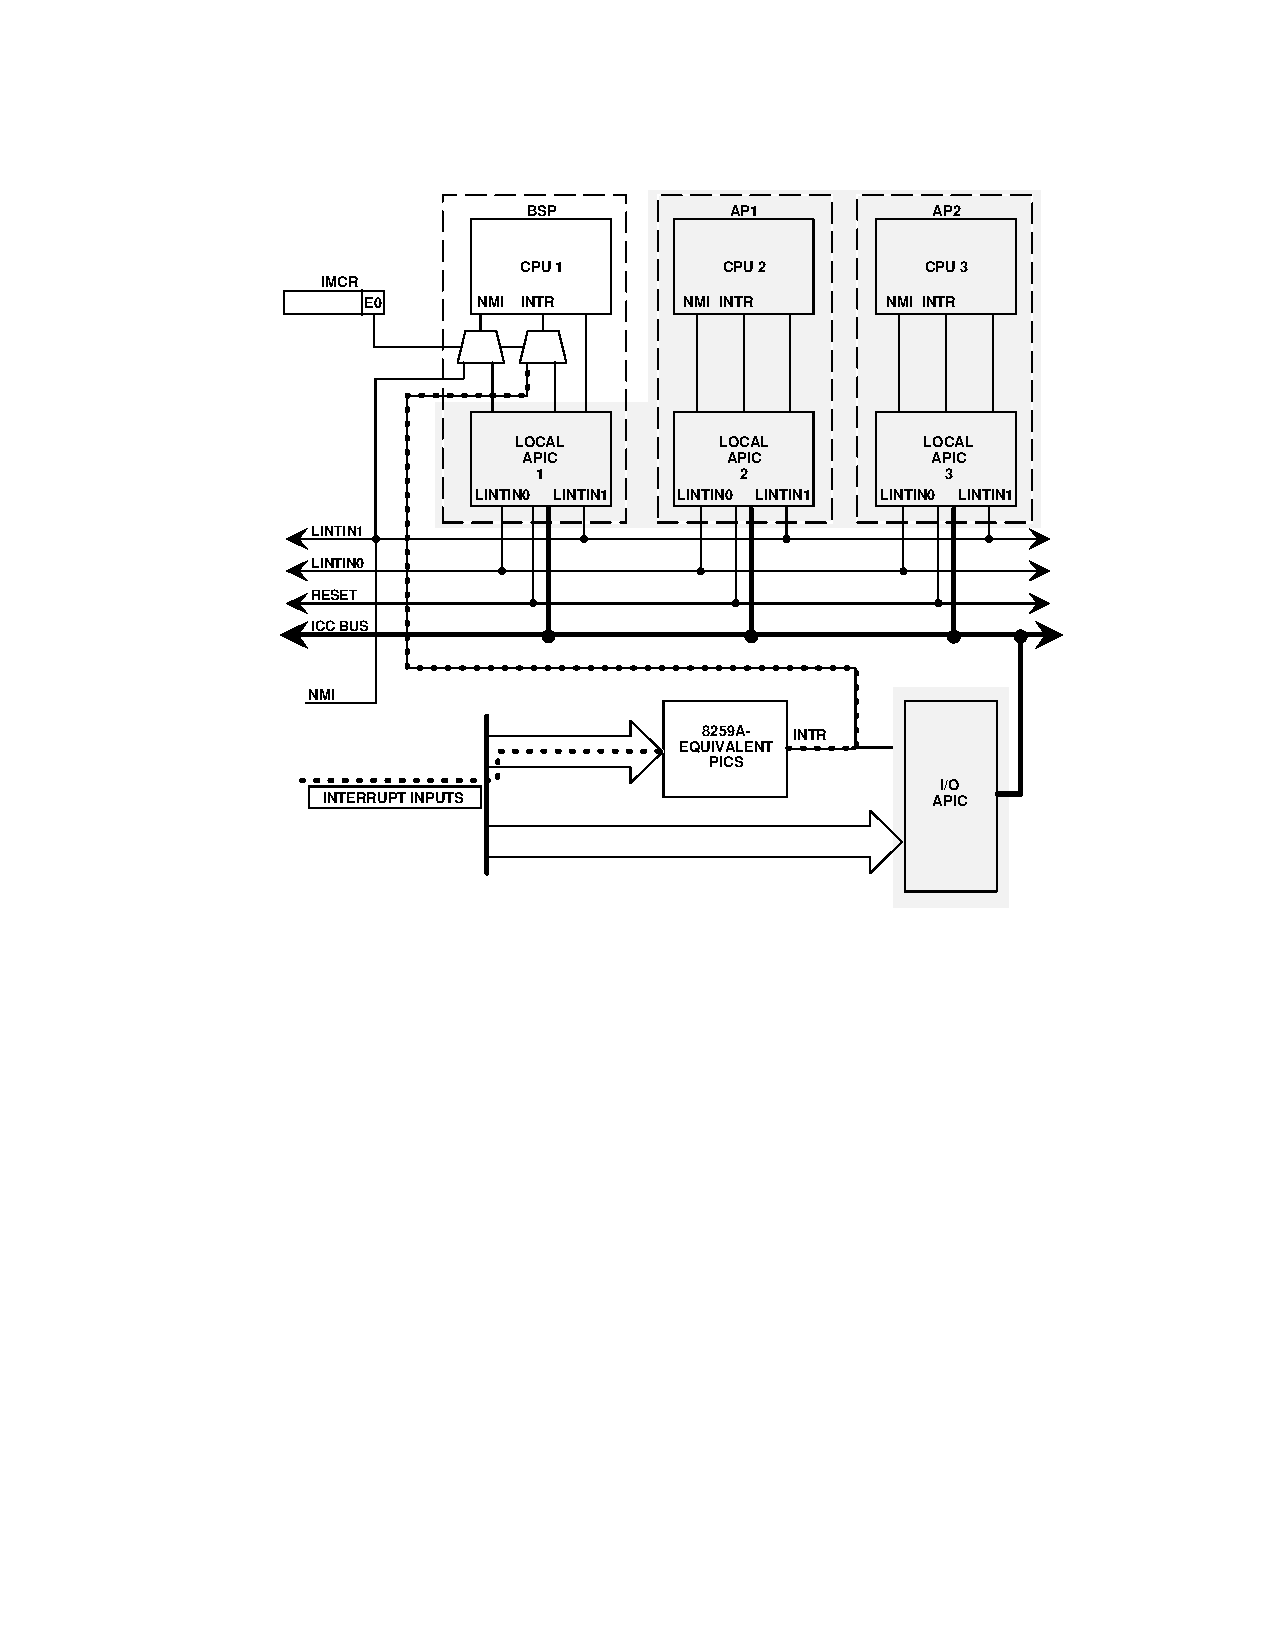
\includegraphics[width=0.9\textwidth]{pic_mode}}
 \caption{PIC interrupt mode} \label{fig:picmode}
\end{figure}

For old version of MP configuration, MP Floating Pointer Structure is employed to provide MP information to the guest OS.   MP Floating Pointer Structure specification is given in  \cite{MP}.

\paragraph{Fake the hardware configuration for Guest OS}
First copy the hardware configuration from the lower memory region. Then modify the new copy of configuration to be of single processor with only PIC.  Last, modify the Nested Page Table for the Guest OS to include this modified copy of configuration as the booted hardware configuration source.

We have already finished the code for PIC simulation.  It will work with interrupt handling (Section \ref{subsec:interrupthandling}) to serve the guest OS.
To support guest OS with multi physical cores, I think we need to later implement the simulation of APIC and IOAPIC.

\subsubsection{Interrupt Handling}
\label{subsec:interrupthandling}
As CertiKOS and Guest OS share some of these physical devices, like keyboard, it requires the CertiKOS to handle some external interrupts for the Guest OS to correctly handle interruption events.

  \begin{figure}[!ht]
 \centerline{
 \includegraphics[width=0.6\textwidth]{interrupt_handle}}
 \caption{Interrupt handling for guest OS} \label{fig:interrupthandle}
\end{figure}
As in Figure \ref{fig:interrupthandle}, CertiKOS intercepts the interrupt events for handling these external interrupts for guest OS.   First, CertiKOS will set the interception setting of the guest domain (Step 1 in Figure \ref{fig:interrupthandle}).  Once the guest has these specified interrupts, the CertiKOS will intercept the event and return the correct IRQ handler for the guest OS (Step 2 in Figure \ref{fig:interrupthandle}). Then the guest can continue its execution for handling the interrupt.

Now we are implementing and testing  the code of interrupt handling for guest OS.

\subsubsection{PCI}
For simplicity, we are now modifying the MP configuration for the guest OS and make guest think that there is no PCI devices.
However, in future, if CertiKOS needs to share PCI devices between the host and guest, we have to implement the simulation of PCI bus and schedule the device accessing.

We are now testing the codes and setting for PCI simulation for the Guest.

\subsection{Working problem}

\subsubsection{Virtualzing Interrupt  based on PIC}

How to virtualize the interrupts based on VPIC  for the guest OS? we are trying to confirm and  check our understanding by  examining the QEMU-KVM and test cases on CertiKOS.  Some of these points that need be further confirmed are presented in following paragraphs.
  \begin{figure}[!ht]
 \centerline{
 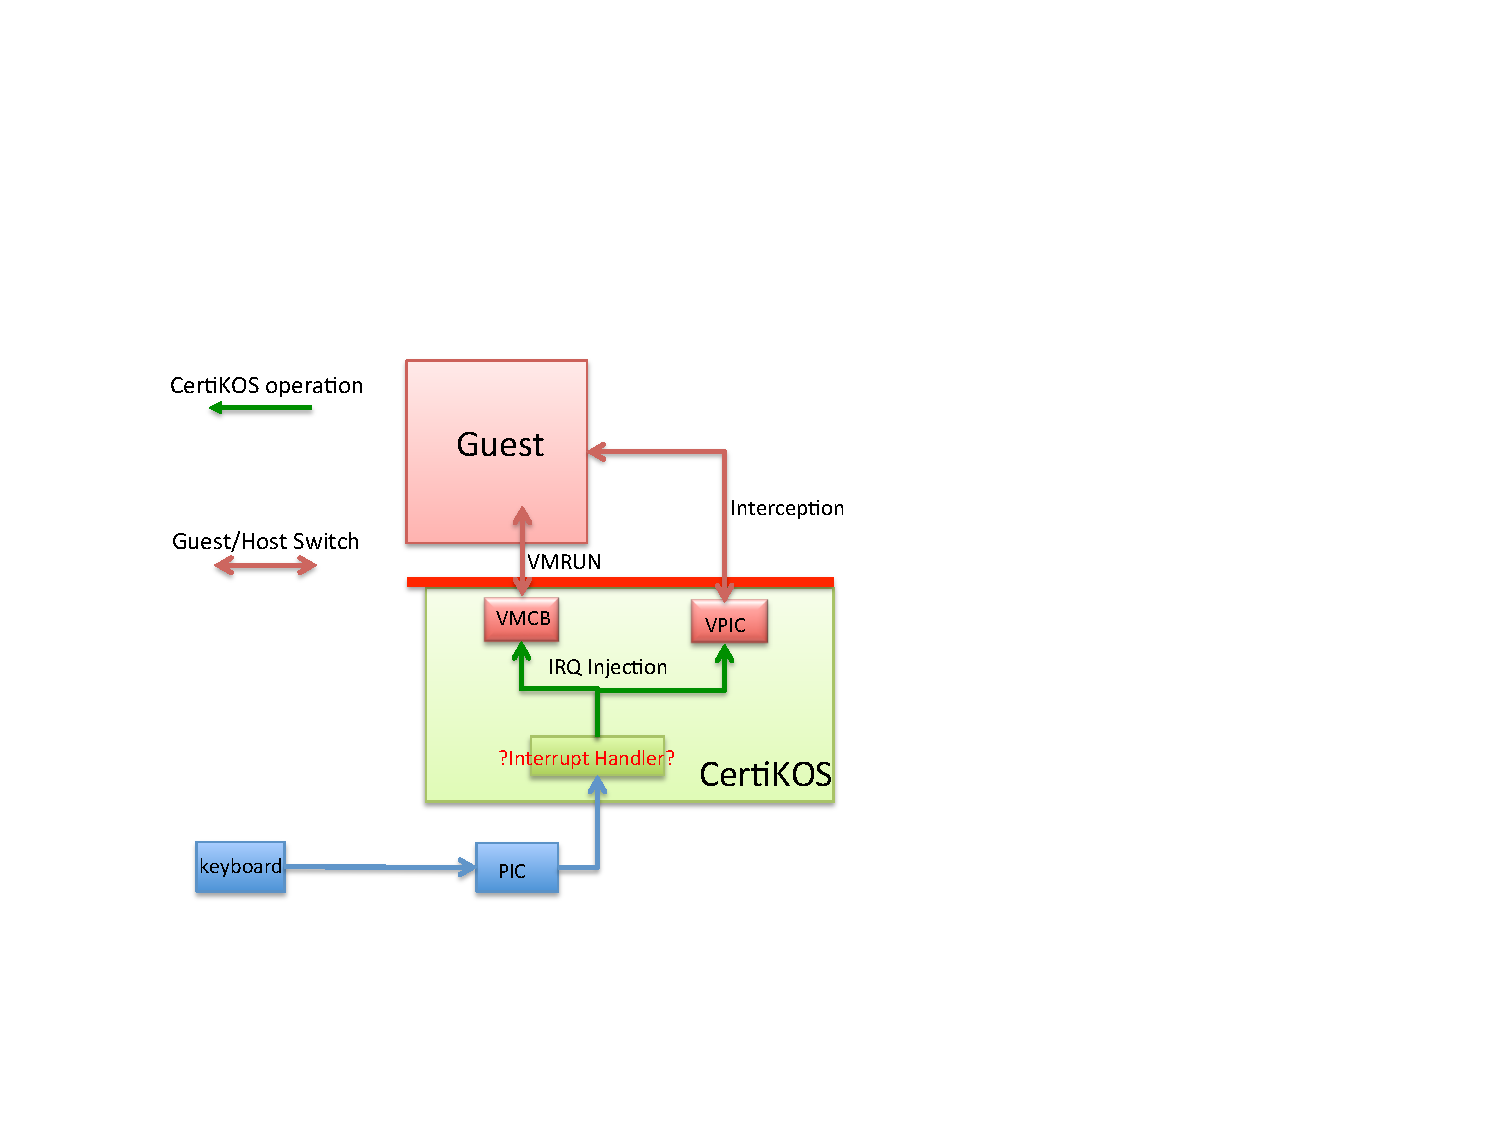
\includegraphics[width=0.6\textwidth]{interrupt_injection}}
 \caption{PIC Interrupt virtualizing for guest OS} \label{fig:interruptinjection}
\end{figure}

When a physical device interrupt happens, like keyboard,  CertiKOS checks whether this is for the guest (By checking the interrupt pending status of the guest). If it is, then CertiKOS will inject Interrupt into guest by setting VMCB of the guest os.   Whether our understanding about virtualizing interrupts correct? 

Where is the right place for the IRQ injection in CertiKOS? The CertiKOS interrupt handler?  In another word, How can CertiKOS separates external interrupt events for its own and guest OS? 

In AMD SVM specification, it introduces a kind of interception for Virtual Interrupts in Guest OS.   I am still not sure whether this type of virtual interrupt is what we want to implement (interrupt virtualization),  or  it refers to the guest OS  interrupts of protected mode virtual interrupt. If it is for interrupt virtualization, how can we leverage it to help the PIC related interrupt simulation?  We are still checking the implementation of KVM to study its usage. 

\subsubsection{Test and Debug CertiKOS on Physical Platform}


\subsection{Target for Current Stage}
We are now mostly working on finish following tasks : 
\begin{itemize}
\item boot ttyLinux as guest OS with CertiKOS on Physical Platform
\item boot ttyLinux with simulated PIC interrupt mode  in CertiKOS
\item intercept  critical operation in ttyLinux
\end{itemize}


\section{Related Work}

\subsection{Interrupt simulation in QEMU and KVM}
$kvm\_arch\_pre\_run$



\bibliographystyle{plain}
\bibliography{certikos}


\end{document}
